\documentclass[12pt]{article}

\usepackage{amsmath, color}
\usepackage{mdwmath}
\usepackage{amssymb, epsf, epsfig, textcomp}
\renewcommand{\baselinestretch}{1.3}
\usepackage{a4wide}
\newcommand{\argmin}{\mathop{\mathrm{argmin}}}
\usepackage{caption}
\usepackage{subcaption}
\usepackage{mathtools}
\usepackage{listings}
\lstdefinestyle{myCustomMatlabStyle}{
	basicstyle=\ttfamily\tiny,
	breaklines=true,
	language=Matlab,
	numbers=left,
	stepnumber=1,
	numbersep=10pt,
	tabsize=4,
	showspaces=false,
	showstringspaces=false
}

\usepackage{sectsty}
\newcommand{\en}{\selectlanguage{english}}	% Set language to english
\newcommand{\el}{\selectlanguage{greek}}	% Set language to greek
\newcommand{\latin}[1]{\en#1\el}			% English text in greek text environment
\newcommand{\code}[1]{\texttt{\latin{#1}}}	% In-line code snippet
\newcommand{\unit}[1]{\text{\latin{ #1}}}	% For upright font in math mode
\newcommand\numberthis{\addtocounter{equation}{1}\tag{\theequation}}

\sectionfont{\fontsize{12}{15}\selectfont}

\begin{document}
	\noindent\rule{\textwidth}{2pt}
	\begin{center}
		{\bf Technical University of Crete}\\
		{\bf School of Electrical and Computer Engineering} \\
		Course: {\bf Convex Optimization} \\
		Exercise 4 (100/1000) \\
		Report Delivery Date: 16 December 2021 \\
		Instructor: Athanasios P. Liavas \\
	\end{center}
	{\bf Student: }Alevrakis Dimitrios 2017030001\\
	\rule{\textwidth}{.5pt}
	\vskip .1cm
	\noindent
	
	Consider the problem:
	\begin{align*}
		&\underset{{\bf x}\in \mathbb{R}^n}{\text{min }}f(x)=-\sum_{i=1}^{n}log(x_i)
		&\text{subject to }{\bf Ax} = {\bf b}
	\end{align*}
	where $\displaystyle {\bf A}\mathbb{R}^p,\ rank({\bf A})=p,\ {\bf b}\in\mathbb{R}^p$.
	\begin{enumerate}
		\item[1.]
		Data Generation. The function rand of MATLAB return a matrix with i.i.d elements with $\mathbb{U}[0,1]$. So for given $n,\ p$ we generate, ${\bf A}~\mathbb{U}[0,1]$ and a ${\bf x}~\mathbb{U}[0,1]$ in order to derive ${\bf b}={\bf A}{\bf x}$.
		
		\item[2.]
		We use cvx to solve the problem. The MATLAB code will be added in the end for possible review.
		
		\item[3.]
		We solved the problem using the Newton algorithm starting from a feasible point.
		\begin{enumerate}
			\item[i.]
			First we find a feasible point using cvx and setting the problem equal to 0 and constraints ${\bf A}{\bf x}={\bf b}$ and ${x>0}$.
			
			\item[ii.]
			We implement the newton algorithm with backtracking line search.
			In each iteration we need to check if the step keeps ${\bf x}$ in the domain of f.
			Also since the problem has affine equality constraints, the KKT for the second order approximation of f can be written as (by taking into account that ${\bf A}{\bf x}=b$ since x is feasible):
			\begin{align*}
				&\nabla^2f(x){\bf \Delta x} + {\bf A}^T{\bf w} + \nabla f(x)=0 \numberthis\\
				&{\bf A}{\bf \Delta x}=0 \numberthis
			\end{align*}
			We solve (1) for ${\bf \Delta x}$:
			\begin{align*}
				\nabla^2f(x){\bf \Delta x} + {\bf A}^T{\bf w} + \nabla f(x)=0 \Rightarrow {\bf \Delta x}=-(\nabla^2f(x))^{-1}({\bf A}^T{\bf w} + \nabla f(x))\numberthis
			\end{align*}
			Substitute (3) to (2):
			\begin{align*}
				&{\bf A}{\bf \Delta x}=0 \Rightarrow -{\bf A}(\nabla^2f(x))^{-1}({\bf A}^T{\bf w} + \nabla f(x))=0\Rightarrow\\
				&-{\bf A}(\nabla^2f(x))^{-1}{\bf A}^T{\bf w}-{\bf A}(\nabla^2f(x))^{-1}\nabla f(x)=0\Rightarrow\\
				&{\bf w}=-({\bf A}(\nabla^2f(x))^{-1}{\bf A}^T)^{-1}{\bf A}(\nabla^2f(x))^{-1}\nabla f(x) \numberthis
			\end{align*}
			
			Also the newton descend which we use for the terminating condition:\\
			$\displaystyle \lambda^2={\bf \Delta x}^T\nabla^2f(x){\bf \Delta x}$
			
			\item[iii.]
			We plot the norm of $x_k$ in each iteration against the solution produced by cvx.
			\begin{figure}[h!]
				\begin{center}
					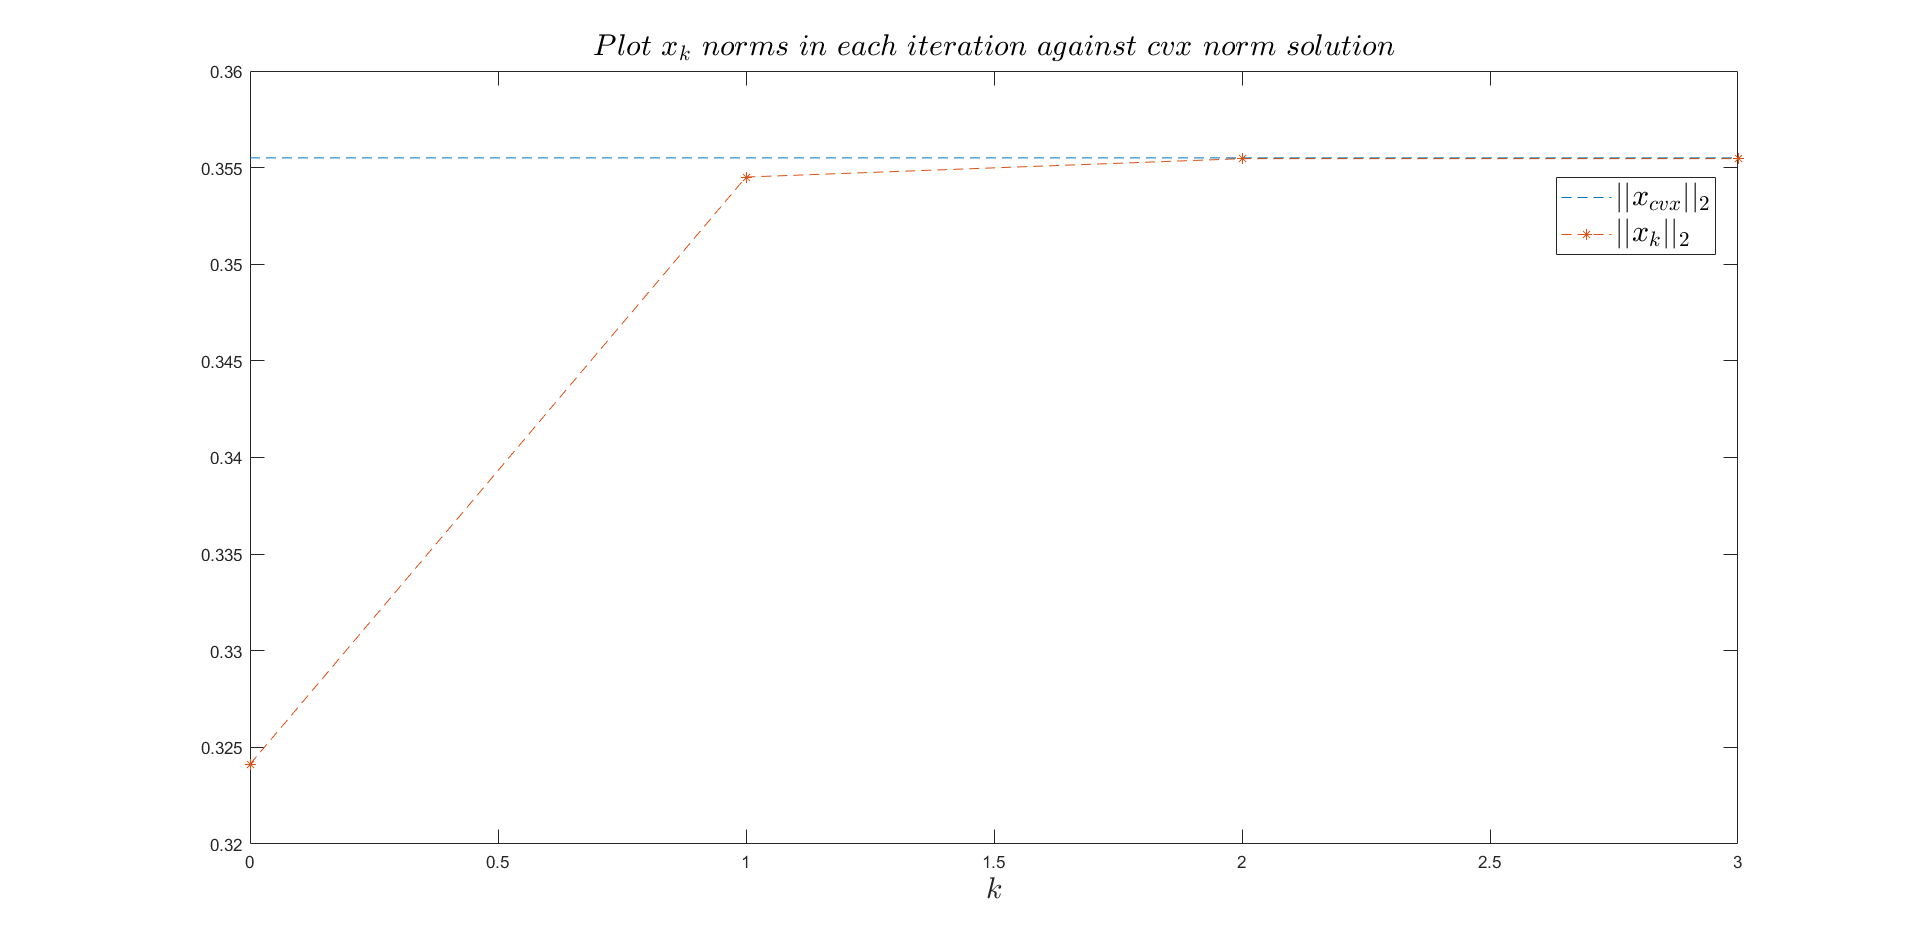
\includegraphics[width=1\linewidth]{2}
				\end{center}
				\caption{Algorithm progression for $n=2,p=1$}
			\end{figure}
			We observe how the $x_k$ gets closer to the solution in each iteration.
		\end{enumerate}
	
		\item[4]
		Again the KKT for the second order approximation of f can be written as:
		\begin{align*}
			&\nabla^2f(x){\bf \Delta x} + {\bf A}^T{\bf v} =-\nabla f(x) \numberthis\\
			&{\bf A}{\bf x}-{\bf b}=0 \numberthis
		\end{align*} 
		Let the residual function $r:\mathbb{R}^n x \mathbb{R}^p \rightarrow \mathbb{R}^n x \mathbb{R}^p$:
		\begin{align*}
			r({\bf x},{\bf v})=(r_{dual}({\bf x},{\bf v}),r_{primal}({\bf x},{\bf v}))
		\end{align*}
		Where the dual residual: $\displaystyle r_{dual}({\bf x},{\bf v})=\nabla f(x) + {\bf A}^T{\bf v}$,\\
		and the primal residual: $\displaystyle r_{primal}({\bf x},{\bf v})={\bf A}{\bf x}-{\bf b}$
		
		By calculating when the first order approximation of $r$ at $({\bf x},{\bf v})$ is equal to 0 we get:
		\begin{align*}
			\begin{bmatrix}
				\nabla^2f(x) & {\bf A}^T\\
				{\bf A} & 0
			\end{bmatrix}
			\begin{bmatrix}
				dx_{pd}\\
				dv_{pd}
			\end{bmatrix}=-
			\begin{bmatrix}
				r_{dual}({\bf x},{\bf v})\\
				 r_{primal}({\bf x},{\bf v})
			\end{bmatrix}=-
			\begin{bmatrix}
				\nabla f(x) + {\bf A}^T{\bf v}\\
				{\bf A}{\bf x}-{\bf b}
			\end{bmatrix}\numberthis
		\end{align*}
		From (7) we get:
		\begin{align*}
			\nabla^2f(x){\bf dx_{pd}}+{\bf A}^T{\bf dv_{pd}}&=-(\nabla f(x) + {\bf A}^T{\bf v})\numberthis\\
			{\bf A}{\bf dx_{pd}}&=-({\bf A}{\bf x}-b)\numberthis
		\end{align*}
		Using (8):
		\begin{align*}
			&(8)\Rightarrow {\bf dx_{pd}}=-(\nabla^2f(x))^{-1}(\nabla f(x) + {\bf A}^T{\bf v}+{\bf A}^T{\bf dv_{pd}}) \Rightarrow\\
			&{\bf A}{\bf dx_{pd}}=-{\bf A}(\nabla^2f(x))^{-1}(\nabla f(x) + {\bf A}^T{\bf v}+{\bf A}^T{\bf dv_{pd}}) \overset{(9)}{\Rightarrow}\\
			&-({\bf A}{\bf x}-b)=-{\bf A}(\nabla^2f(x))^{-1}(\nabla f(x) + {\bf A}^T{\bf v}+{\bf A}^T{\bf dv_{pd}})\\
			&{\bf dv_{pd}}=-({\bf A}(\nabla^2f(x))^{-1}{\bf A}^T)^{-1}\big[{\bf A}(\nabla^2f(x))^{-1}(\nabla f(x) + {\bf A}^T{\bf v})-({\bf A}{\bf x}-{\bf b})\big]
		\end{align*}
	
		Therefore we have calculated the primal-dual steps and can apply the newton algorithm with backtracking line search on $r$.\\
		Since $({\bf dv_{pd}},{\bf dx_{pd}})$ is a descend direction for $||r||_2^2$  we can use $||r({\bf x},{\bf v})||<\epsilon$ as stop criterion for the newton algorithm.
		
		\item[5.]
		Let the Langragian $L:domfx\mathbb{R}^p\rightarrow \mathbb{R}$ where:
		\begin{align*}
			L({\bf x},{\bf v})=-\sum_{i=1}^{n}log(x_i)+{\bf v}^T({\bf A}{\bf x}-{\bf b})
		\end{align*}
		Therefore the dual problem is:
		\begin{align*}
			\underset{{\bf v}\in \mathbb{R}^p}{max}\underset{{\bf x\in domf}}{min}L({\bf x},{\bf v})
		\end{align*}
		and the dual function is defined as:
		\begin{align*}
			g({\bf v})=\underset{{\bf x\in domf}}{inf} L({\bf x},{\bf v})
		\end{align*}.
	
		We will prove that L for a given ${\bf v}$ is convex:\\
		The gradient of f:
		\begin{align*}
			\nabla_{\bf x} L({\bf x},{\bf v})_i=-\frac{1}{x_i}+({\bf A}^T{\bf v})_i,\ i=1,...,n
		\end{align*}
		and the hessian:
		\begin{align*}
			\nabla_{\bf x}^2 L({\bf x},{\bf v})=diag(\frac{1}{x^2_i}),\ i=1,...,n
		\end{align*}
		If the hessian is positive definite then L is convex:\\
		Let ${\bf z}\in\mathbb{R}^n-{\bf 0}$
		\begin{align*}
			{\bf z}^T\nabla_{\bf x}^2 L({\bf x},{\bf v}){\bf z}= (z_i)^2\frac{1}{x^2_i} >0 \forall {\bf z}\in\mathbb{R}^n-{\bf 0}
		\end{align*}
	
		Since L is convex for a given ${\bf v}$ then we can minimize it by:
		\begin{align*}
			\nabla_{\bf x}L({\bf x},{\bf v})=0 \iff {\bf x_i} = \frac{1}{({\bf A}^T{\bf v})_i}\numberthis
		\end{align*}
	
		Therefore the dual problem is:
		\begin{align*}
			maximize g(v)=\underset{{\bf x}}{inf}L({\bf x},{\bf v})=\sum_{i=1}^{n}log({\bf A}^T{\bf v})_i+n-{\bf b}^T{\bf v}
		\end{align*}
		We now use cvx to solve the dual and via (10) we calculate the primal.
		
		\item[6.]
		\begin{figure}[h!]
			\begin{center}
				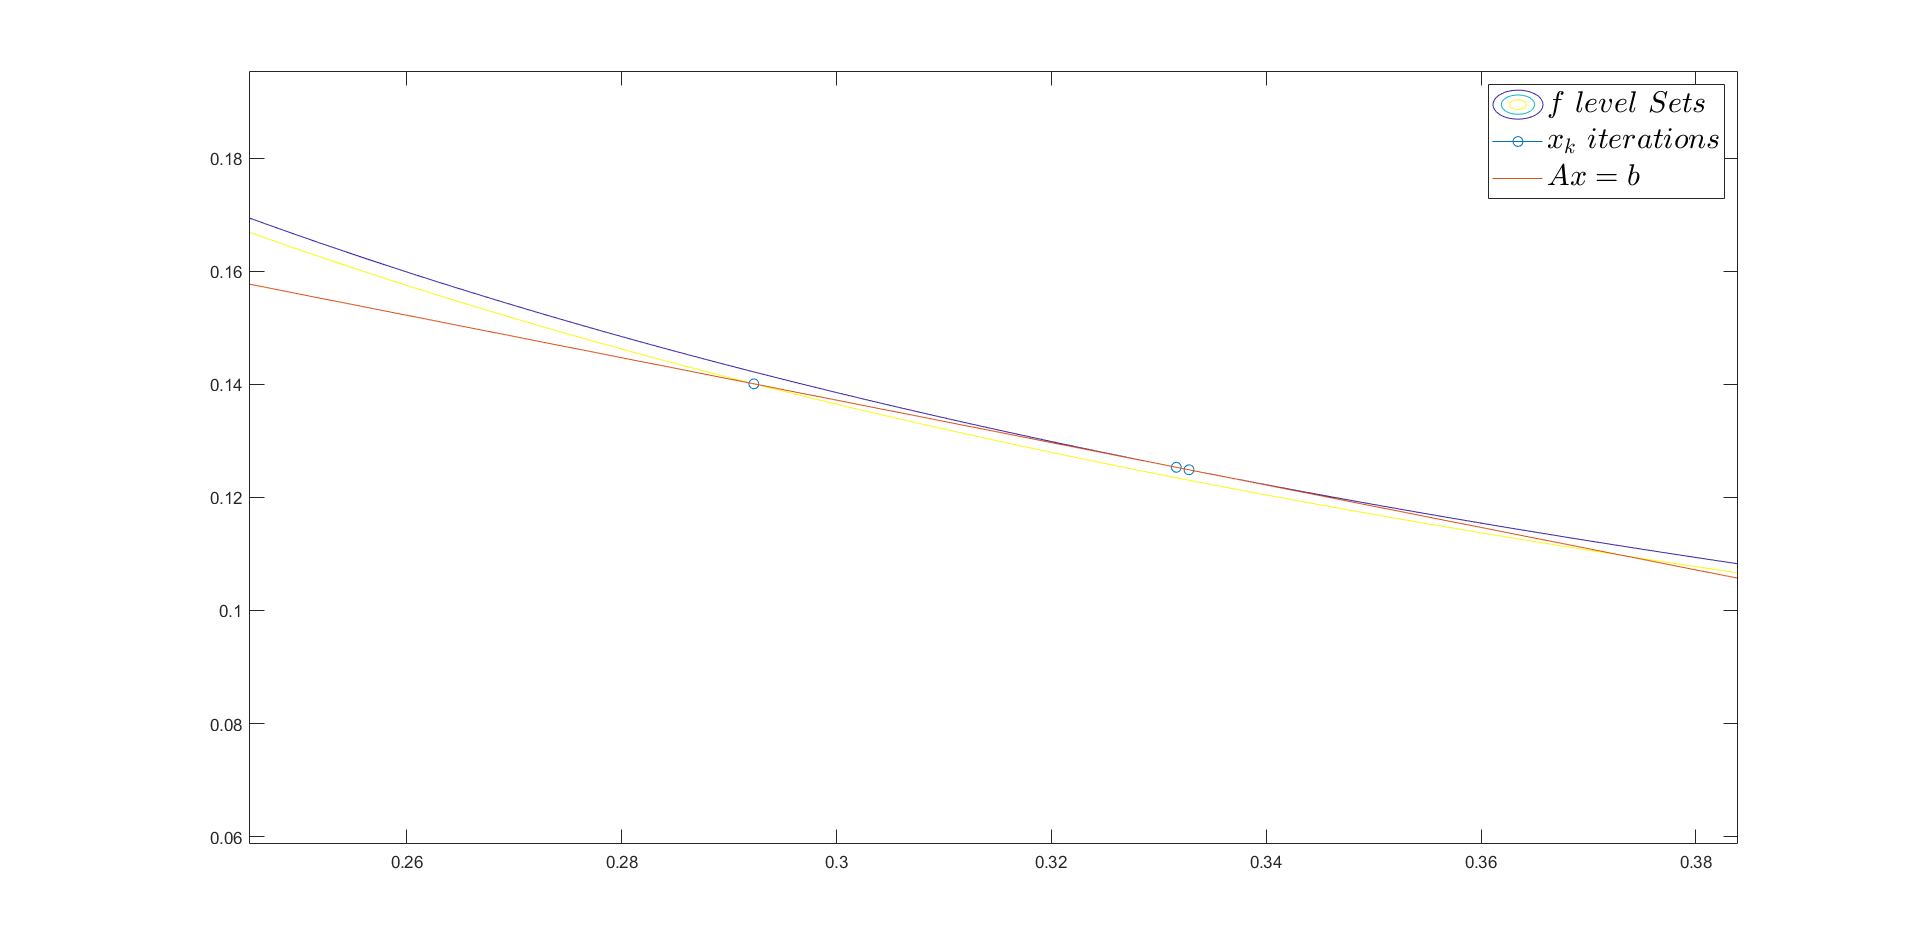
\includegraphics[width=\linewidth]{1}
			\end{center}
			\caption{${\bf A}{\bf x}={\bf b}$, f level sets and newton algorithm progress starting from feasible point}
		\end{figure}
		\begin{figure}[h!]
			\begin{center}
				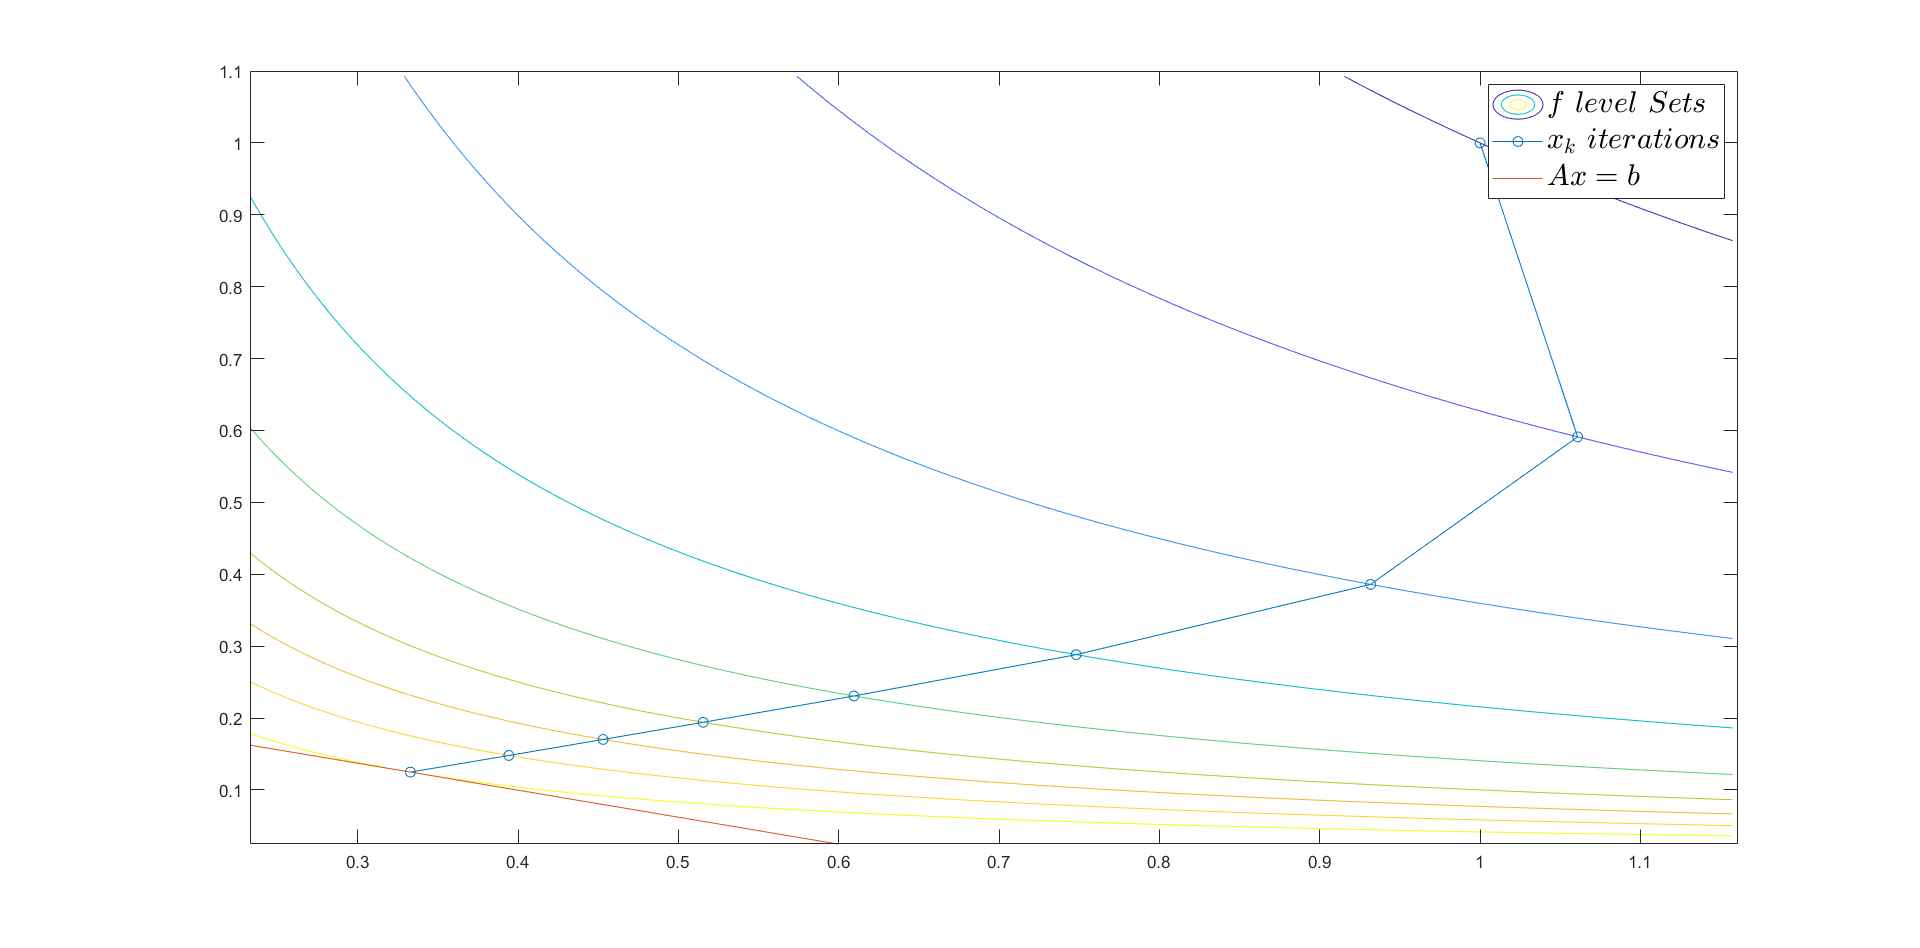
\includegraphics[width=\linewidth]{3}
			\end{center}
			\caption{${\bf A}{\bf x}={\bf b}$, f level sets and primal-dual algorithm progress with starting from infeasible point}
		\end{figure}
		We observe how in figure 2 the iterations always stay feasible and on ${\bf A}{\bf x}={\bf b}$, while in figure 3 we start from from an infeasible point and approach ${\bf A}{\bf x}={\bf b}$.\\
		\newpage
		{\bf Exercise4.m}: This script contains the code for the execution of the above.
		\lstinputlisting{Exercise4.m}
	\end{enumerate}
\end{document}
